%% LyX 1.6.2 created this file.  For more info, see http://www.lyx.org/.
%% Do not edit unless you really know what you are doing.
\documentclass[12pt,english]{article}
\usepackage{mathptmx}
\renewcommand{\familydefault}{\rmdefault}
\usepackage[T1]{fontenc}
\usepackage[latin9]{inputenc}
\usepackage[letterpaper]{geometry}
\geometry{verbose,tmargin=1cm,bmargin=2cm,lmargin=1cm,rmargin=1cm,headheight=1cm,headsep=1cm,footskip=1cm}
\setlength{\parskip}{\medskipamount}
\setlength{\parindent}{0pt}
\usepackage{graphicx}


%%%%%%%%%%%%%%%%%%%%%%%%%%%%%% LyX specific LaTeX commands.
%% Because html converters don't know tabularnewline
\providecommand{\tabularnewline}{\\}

\usepackage{babel}

\begin{document}

\part*{Kunst}

\begin{tabular}{|c|c|}
\hline 
Kurs & Kunst\tabularnewline
\hline
\hline 
Lehrer/Lehrerin & Frau Schmidt\tabularnewline
\hline 
Zeitraum & Sommer 2008 bis Sommer 2009\tabularnewline
\hline 
Klassenstufe & Einf�hrungsphase\tabularnewline
\hline
\end{tabular}


\section*{03.02.09}

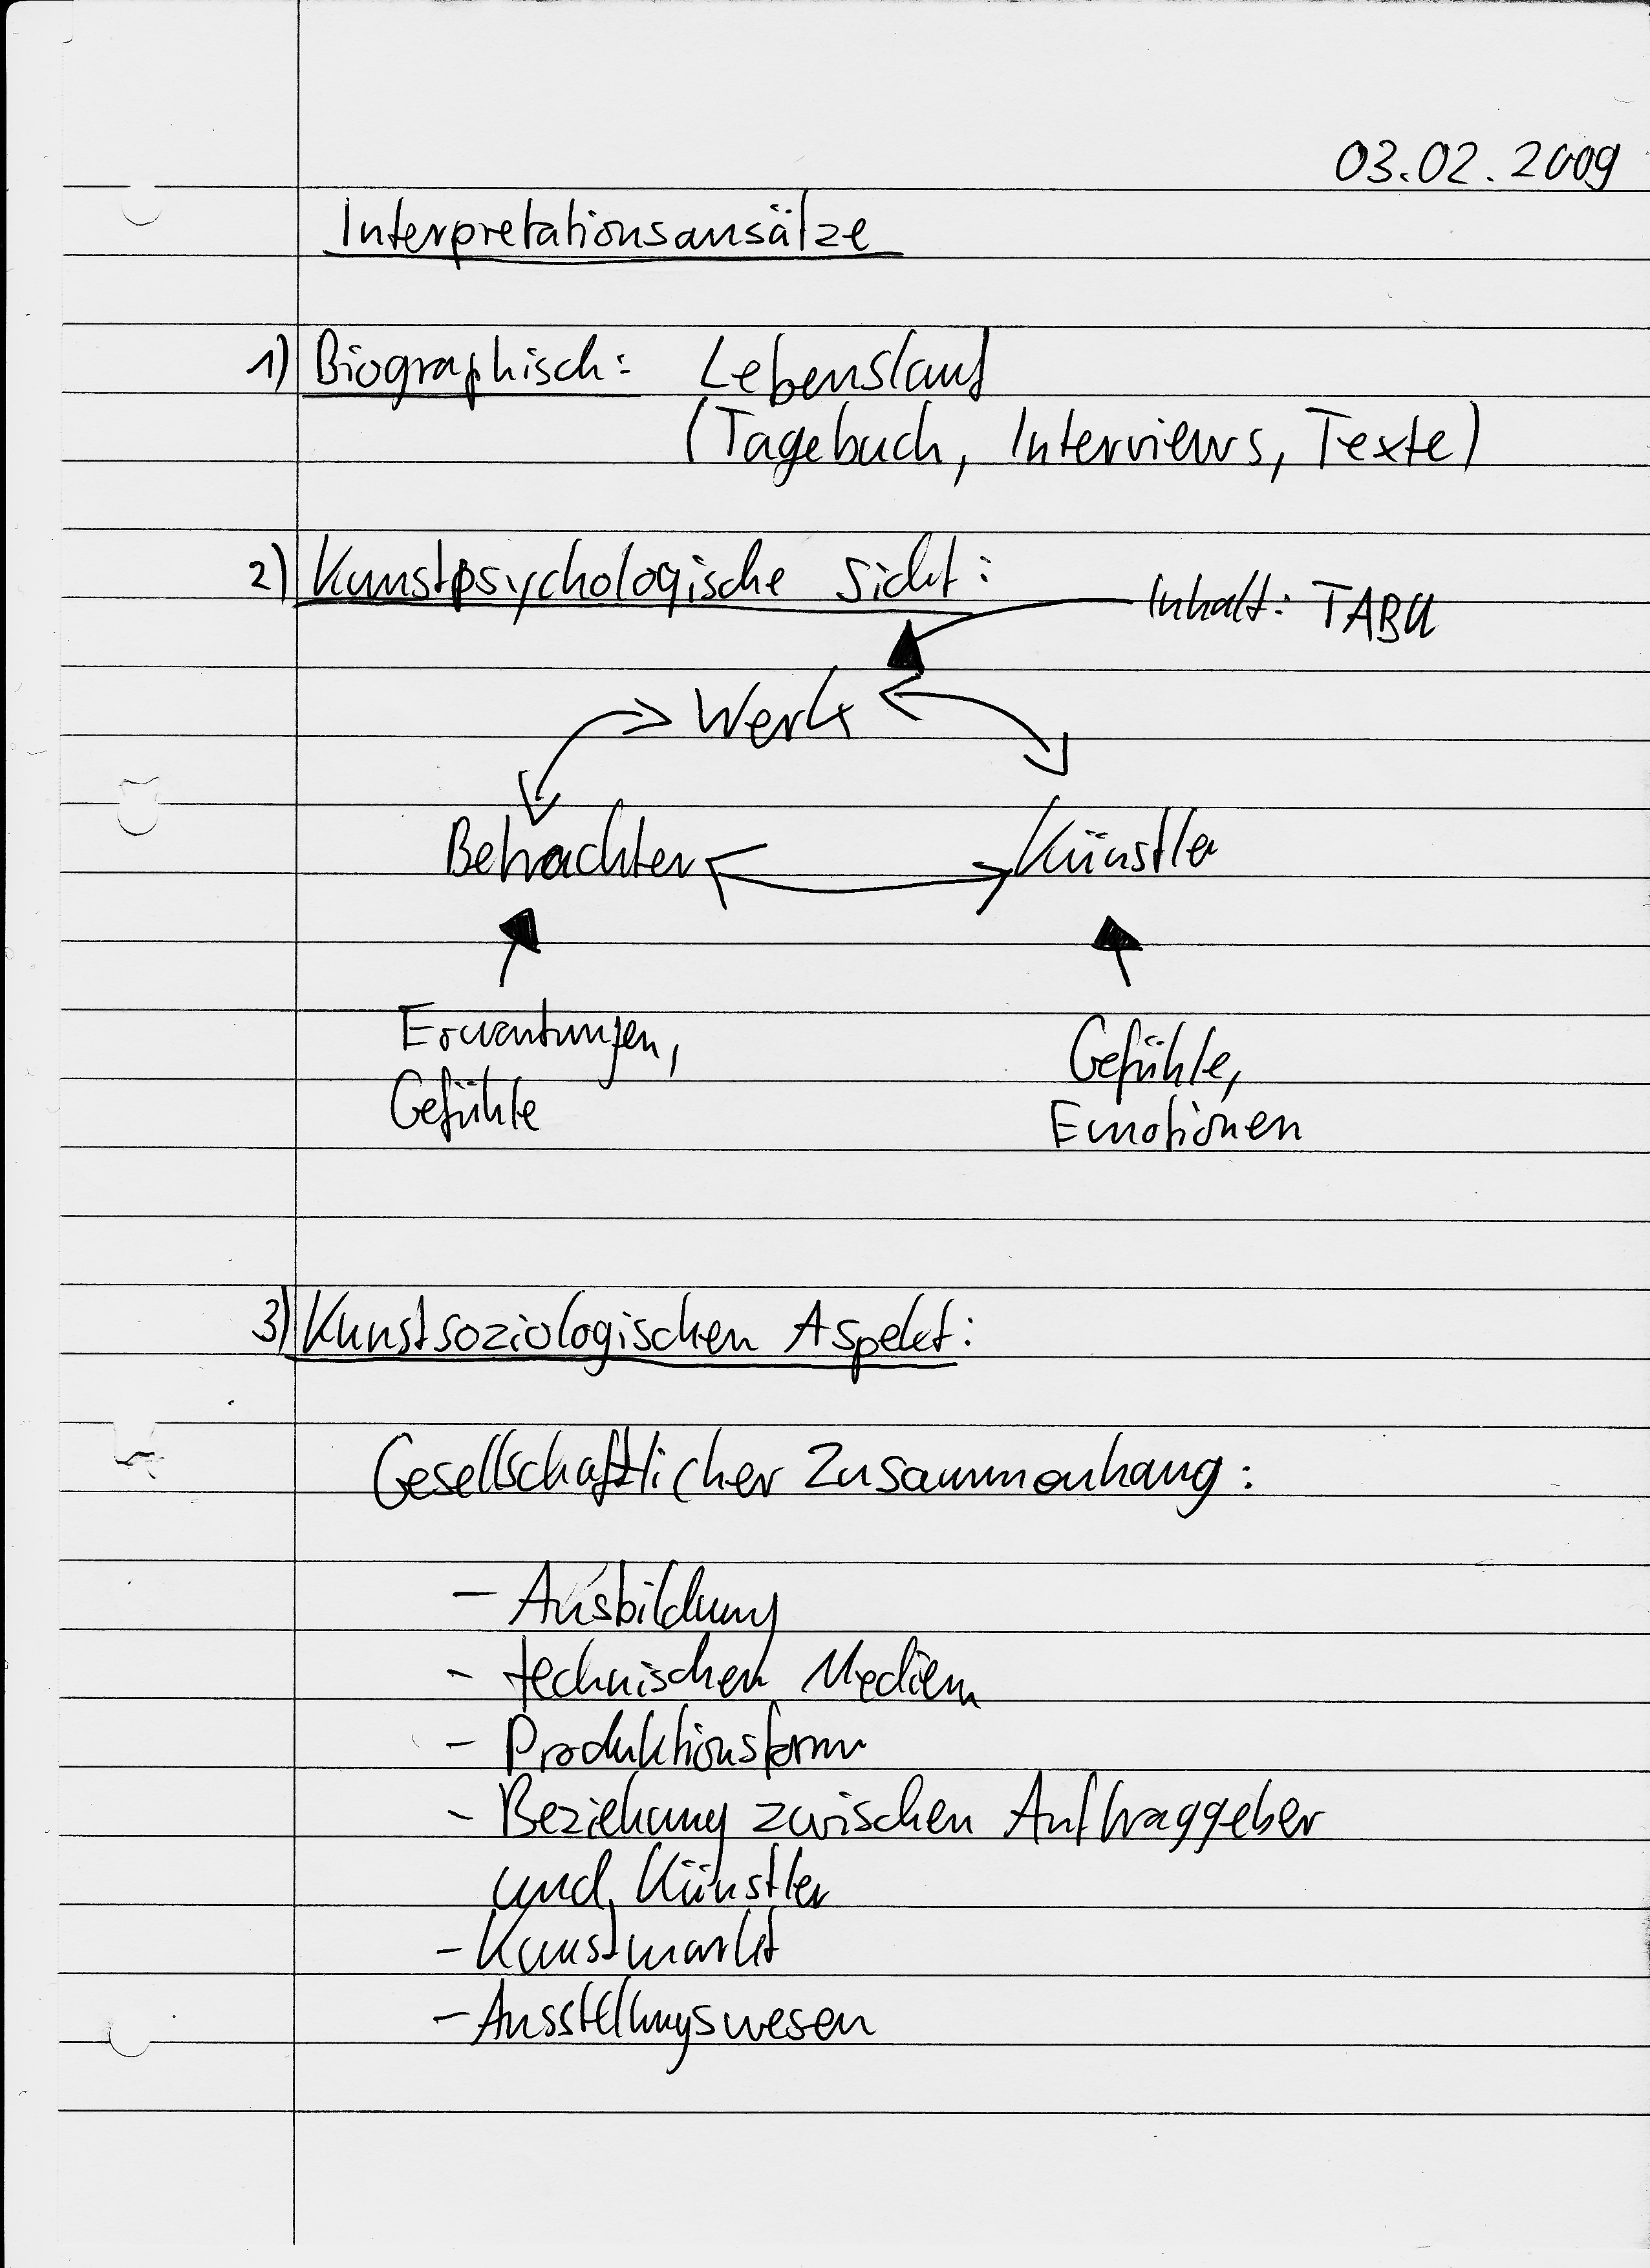
\includegraphics[width=0.8\paperwidth]{2009-02-09_Interpretationsansaetze}

\includegraphics[width=0.8\paperwidth]{\string"2009-02-09_Zeitplan zweites Halbjahr\string".eps}

\includegraphics[width=0.8\paperwidth]{\string"2009-02-09_Kunst Portfolio zweites Halbjahr\string".eps}


\section*{10.02.09}


\subsection*{Interpretationsans�tze}
\begin{enumerate}
\item Strukturanalyse:

\begin{enumerate}
\item Kunstwerk und seine einzelnen Elemente
\end{enumerate}
\item Stilanalyse:

\begin{enumerate}
\item vergleicht verschiedene Kunstwerke

\begin{enumerate}
\item Zeitstil
\item Nationalstil
\item Individualstil
\end{enumerate}
\end{enumerate}
\item Ikonografische Interpretation:

\begin{enumerate}
\item = die Lehre von den Bildinhalten (Symbole etc.)
\end{enumerate}
\item Ikonologische Interpretation:

\begin{enumerate}
\item Zeitdimension: {}``Was sagt mir heute das Bild?''
\end{enumerate}
\item Rezeptions�sthetische Interpretation:

\begin{enumerate}
\item Wahrnehmung des Kunstwerks im Kontext
\end{enumerate}
\end{enumerate}

\end{document}
